\subsection{Simulation Results Using a Single Agent and One Target}\label{subsec:SingleAgentSingleSourceResults}


\begin{landscape}
\centering
\vspace*{\fill}
\begin{table}[h!]
  \centering
  \begin{tabular}{ | c | c | }
    \hline
    Histogram & Parameters/Statistics \\
    \hline
     \multicolumn{2}{c}{Initial Uniform Distribution of Belief Over Grid Cells}\\
    \hline
    %single UAV
    %\begin{minipage}[c][height][c]{width}
    \begin{minipage}[c][40mm][c]{.45\textwidth}
      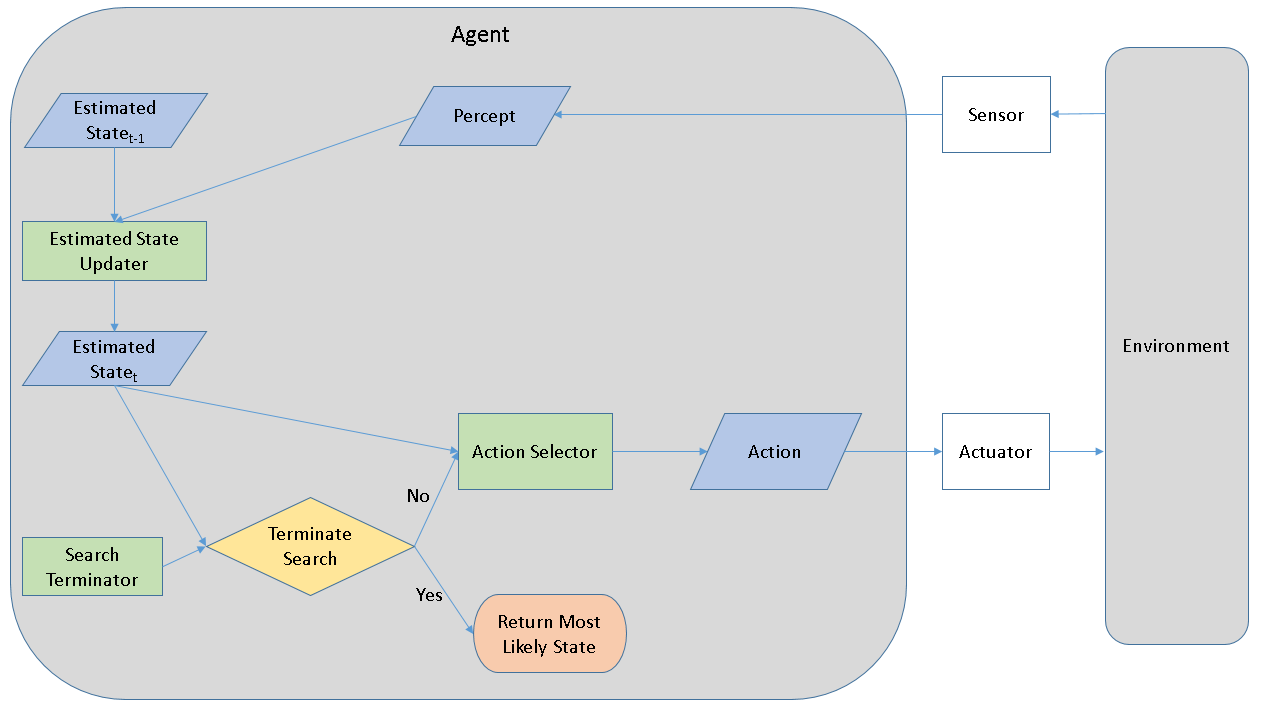
\includegraphics[width=\linewidth, height=38mm]{Chapters/MultiAgentTargetDetection/Figs/AgentFnArchitecture/BasicAgentFunctionNoCommunication.PNG}

    \end{minipage}
    &
    \small
    \begin{tabular}{c|c|c|c|c|c|c|c}
        Strategy & p(T \Romannum{1}) & p(T \Romannum{2}) & Sim. FPR & Sim. FNR & E[TTD] & Prec. & Rec. \\
        \hline
        $\epsilon$ -Greedy & 0.2 & 2 & 0.05 & 233.2 & 2303.3 & 2 & 9\\
        Sweep & 4 & 2 & 0.05 & 233.2 & 2303.3 & ToDo & ToDo\\
        Saccadic & 4 & 2 & 0.05 & 233.2 & 2303.3 & ToDo & ToDo\\
        Random & 4 & 2 & 0.05 & 233.2 & 2303.3 & ToDo & ToDo\\
        Sweep & 4 & 2 & 0.05 & 233.2 & 2303.3 & ToDo & ToDo\\
    \end{tabular}
    \normalsize
    \\
    \hline
    \multicolumn{2}{c}{Initial Discretised Gaussian Distribution of Belief Over Grid Cells (random mean, covariance matrix = [[], []]}\\
    \hline
    %single UAV
    %\begin{minipage}[c][height][c]{width}
    \begin{minipage}[c][40mm][c]{.45\textwidth}
      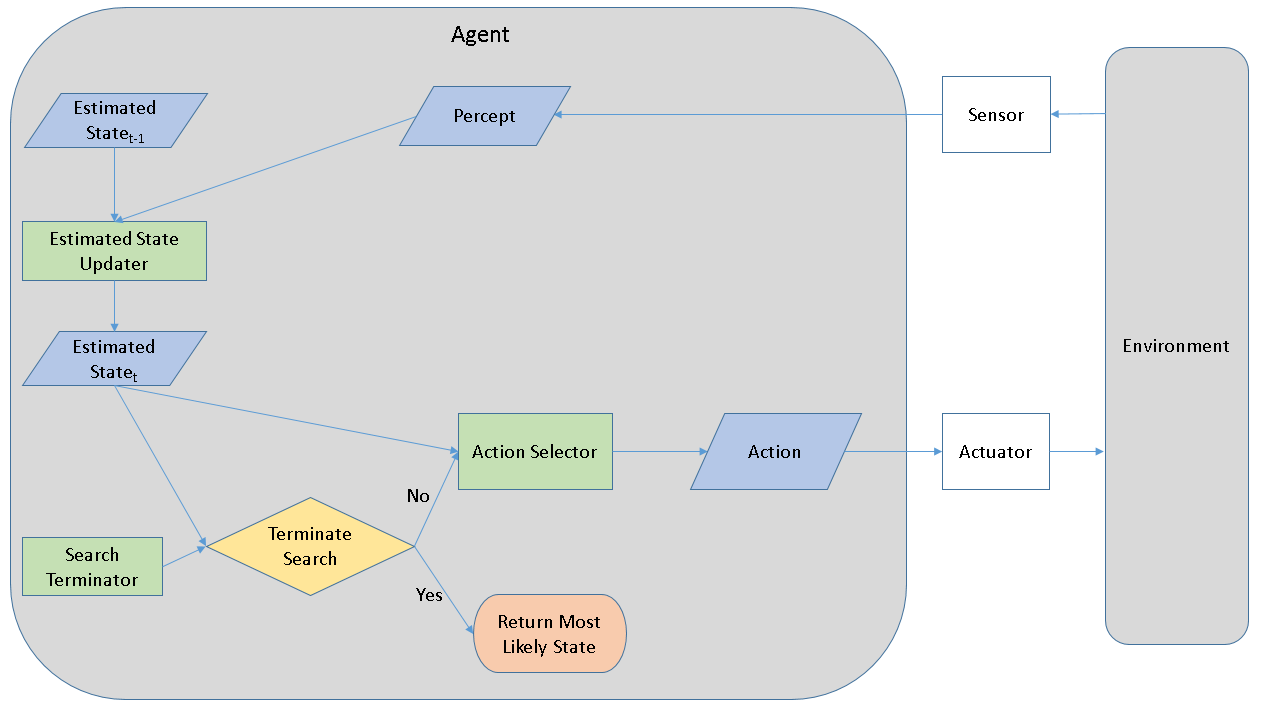
\includegraphics[width=\linewidth, height=38mm]{Chapters/MultiAgentTargetDetection/Figs/AgentFnArchitecture/BasicAgentFunctionNoCommunication.PNG}

    \end{minipage}
    &
    \small
    \begin{tabular}{c|c|c|c|c|c|c|c}
        Strategy & p(T \Romannum{1}) & p(T \Romannum{2}) & Sim. FPR & Sim. FNR & E[TTD] & Prec. & Rec \\
        \hline
        $\epsilon$ -Greedy& 4 & 2 & 0.05 & 233.2 & 2303.3 & 2 & 9\\
        Sweep & 4 & 2 & 0.05 & 233.2 & 2303.3 & 2 & 9\\
        Saccadic & 4 & 2 & 0.05 & 233.2 & 2303.3 & 2 & 9\\
        Random & 4 & 2 & 0.05 & 233.2 & 2303.3 & 2 & 9\\

    \end{tabular}
    \normalsize
    \\
    \hline
   
  \end{tabular}
  \caption{Results of running the target localisation simulation with a  uniform initial belief distribution and Gaussian initial belief distribution. p(T \Romannum{1}) = The probability of making a type \Romannum{1} error using the SPRT, p(T \Romannum{2}) = The probability of making a type \Romannum{1} error using the SPRT, Sim. FPR = The simulated false positive rate of the sensor, Sim. FNR = The simulated false negative rate of the sensor, E[TTD] = The expected amount of timesteps until a decision is made, Prec. = precision, Rec. = Recall. }\label{table:ORToolsResults}
\end{table}
\end{landscape}



\textbf{Uniform Initial Belief Distribution}
%\begin{landscape}
%\centering
%\vspace*{\fill}
\begin{table}[h!]
  \centering
    \begin{tabular}{|c|c|c|c|c|c|}
    \hline
        Strategy & Initial Bel.Target Present & E[TTD] & S.D. T.T.D & FNR. & Prop. Incorrect Locs \\
        \hline
        $\epsilon$ -Greedy & 0.5 & 112.93 & 62.38 & 0.152 & 0.040 \\
        Sweep & 0.5 & 601.57 & 183.45& 0.1254 & 0.0454 \\
        Saccadic & 0.5 & 98.83 & 56.13 & 0.1588 & 0.037 \\
        Random & 0.5 & 629.55 & 282.95 & 0.1368 & 0.0336 \\
        \hline
    \end{tabular}
    \caption{Results of running the target localisation simulation with a  uniform initial belief distribution. Fixed P(T1) = 0.1, p(T2) = 0.15, Simulated Sensor FPR = 0.2, Simulated Sensor FNR = 0.15, Sensor Model FPR = 0.2, Sensor Model FNR = 0.15, }
    \label{table:PriorUniform}
\end{table}
    
   

%    \hline
%    \multicolumn{2}{c}{Initial Discretised Gaussian Distribution of Belief Over Grid Cells (random mean, covariance matrix = [[], []]}\\
%    \hline

\textbf{Gaussian Initial Belief Distribution (Mean coinciding with true target location)}
\begin{table}[h!]
    \centering
    \begin{tabular}{|c|c|c|c|c|c|}
    \hline
       Strategy & Initial Bel.Target Present & E[TTD] & S.D. T.T.D & FNR. & Prop. Incorrect Locs \\
        \hline
        $\epsilon$ -Greedy & 0.5 & 21.68 & 20.44 & 0.0296 & 0.0118 \\
        Sweep & 0.5 & 464.48 & 185.54 & 0.0832 & 0.0294 \\
        Saccadic & 0.5 & 14.558 & 18.75 & 0.0338 & 0.0114 \\
        Random & 0.5 & 501.83 & 268.45 & 0.0792 & 0.0308 \\
    \hline
    \end{tabular}

  \caption{Results of running the target localisation simulation with a  uniform initial belief distribution and Gaussian initial belief distribution. p(T \Romannum{1}) = The probability of making a type \Romannum{1} error using the SPRT, p(T \Romannum{2}) = The probability of making a type \Romannum{1} error using the SPRT, Sim. FPR = The simulated false positive rate of the sensor, Sim. FNR = The simulated false negative rate of the sensor, E[TTD] = The expected amount of timesteps until a decision is made, Prec. = precision, Rec. = Recall. }\label{table:PriorGaussian}
\end{table}


\textbf{Varying Initial Belief in Target Presence in Retion}
\begin{table}[h!]
    \centering
    \begin{tabular}{|c|c|c|c|c|c|}
    \hline
       Strategy & Initial Bel.Target Present & E[TTD] & S.D. T.T.D & FNR. & Prop. Incorrect Locs \\
        \hline
        $\epsilon$ -Greedy & 0.2 & 21.68 & 20.44 & 0.0296 & 0.0118 \\
        $\epsilon$ -Greedy & 0.5 & 112.93 & 62.38 & 0.152 & 0.040 \\
        $\epsilon$ -Greedy & 0.8 & 21.68 & 20.44 & 0.0296 & 0.0118 \\
        
        Sweep & 0.2 & 464.48 & 185.54 & 0.0832 & 0.0294 \\
        Sweep & 4 & 2 & 0.05 & 233.2 & 2303.3 & 2 & 9\\
        Sweep & 0.8 & 464.48 & 185.54 & 0.0832 & 0.0294 \\

        Saccadic & 0.2 & 14.558 & 18.75 & 0.0338 & 0.0114 \\
        Saccadic & 0.5 & 98.83 & 56.13 & 0.1588 & 0.037 \\
        Saccadic & 0.8 & 14.558 & 18.75 & 0.0338 & 0.0114 \\
        
        Random & 0.2 & 501.83 & 268.45 & 0.0792 & 0.0308 \\
        Random & 0.5 & 629.55 & 282.95 & 0.1368 & 0.0336 \\
        Random & 0.2 & 501.83 & 268.45 & 0.0792 & 0.0308 \\

    \hline
    \end{tabular}

  \caption{Results of running the target localisation simulation with a  uniform initial belief distribution and Gaussian initial belief distribution. p(T \Romannum{1}) = The probability of making a type \Romannum{1} error using the SPRT, p(T \Romannum{2}) = The probability of making a type \Romannum{1} error using the SPRT, Sim. FPR = The simulated false positive rate of the sensor, Sim. FNR = The simulated false negative rate of the sensor, E[TTD] = The expected amount of timesteps until a decision is made, Prec. = precision, Rec. = Recall. }\label{table:PriorGaussian}
\end{table}